\documentclass{article}
\usepackage{amsmath}
\usepackage{amsfonts}
\usepackage{graphicx}
\usepackage[frenchb]{babel}
\usepackage[utf8]{inputenc}
\usepackage[left=.8in, right=.8in, top=.8in, bottom=.8in]{geometry}

\title{\textsc{Rapport projet ASCII Art}}
\date{}

\begin{document}

\maketitle
\begin{center}

\includegraphics[height=8cm]{enseirblogo.png}
\end{center}

\section{Présentation du problème}
L'ASCII Art est une technique d'informatique utilisée pour représenter une image en caractères ASCII (caractères d'écriture).
\newline
\begin{figure}[h]
\centering
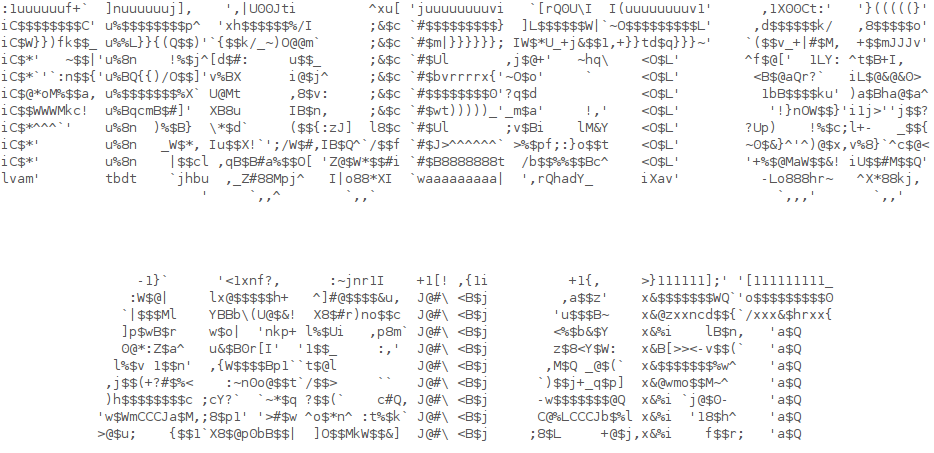
\includegraphics[width=8cm]{ascii_art_s5.png}
\caption{Exemple d'un ASCII Art.}
\end{figure}

Le but du projet ASCII Art est de réaliser un programme qui, partant d'une image dans un format quelconque, pourra la représenter en ASCII dans différents formats (noir et blanc, niveau de gris, et en couleurs). La majeure partie du travail de l'algorithme sera commun aux trois formats. De plus, les formats couleur et niveaux de gris auront eux-même deux sous-formats, selon qu'on souhaite l'image en trames ou en caractères ASCII.
\newline

\section{Travail algorithmique}
Le ligne de commande pour lancer l'execution du programme contient le nom de l'exécutable, le chemin vers le fichier à transformer, et le type de transformation qu'on veut lui appliquer (type 0, 1, 2, 3 ou 4). Le programme prend en compte cette deuxième information pour choisir quelle est la partie du code à utiliser.Les cinq différentes transformations sont : noir et blanc (0), caractères ASCII en niveaux de gris (1), caractères ASCII en couleur(2), trames en niveaux de gris (3), trames en couleur (4). L'utilisateur peut exporter le résultat sous forme d'un fichier HTML s'il le souhaite.
\newline

En premier lieu, on va générer le fichier de travail, en créant une chaîne de caractères qui sera, en fait, la ligne de commande à exécuter dans le terminal. Une grande partie est commune aux cinq cas, et la différence se fait grâce à un case. Si l'image est souhaitée en noir et blanc, on convertit en pbm (on rajoute donc un .pbm à la fin de la ligne de commande), si c'est en niveau de gris, on convertit en pgm, et enfin en couleur, en ppm. 
\newline

Quelque soit le type du fichier, il commence de la même manière : la première ligne contient le "nombre magique" qui permet de déterminer à quel genre de transformation on a affaire, et la deuxième ligne est la taille de l'image. On va récupèrer cette taille, divisée en deux dimensions (largeur et longueur), dans une structure nécessaire au bon affichage final. 
\newline

A noter que, pour des choix de propreté d'affichage, l'image sera redimensionnée lors de la conversion en fichier pbm, pgm ou ppm : sa largeur est multipliée par 1.3, ceci pour contrer l'effet d'amaigrissement causé par la transformation en caractères.
\newline

Ensuite on stocke le reste du fichier dans un tableau d'entiers, qui selon le type de la transformation, contiendra soit des 0 et 1 (pbm), des nombres entre 0 et 255 (pgm)  ou une succession de trois nombres représentant le niveau en rouge, vert et bleu (ppm). 

\subsection{Type de transformation 0 : Noir et blanc}
Dans le cas d'une image finale en noir et blanc, le fichier pbm est uniquement constitué de 1 et de 0, les premiers représentant les pixels noirs et les autres les pixels blancs. Grâce aux dimensions, connues, de l'image, on va stocker toutes ces valeurs dans un tableau suffisamment grand (après conversion des caractères du fichier en entiers). 
\newline

Les pixels vont être étudiés par groupes de quatre (blocs de 2 x 2 pixels). A partir du tableau d'entiers, cela se fait modulo la largeur de l'image : on récupère dans un tableau de taille quatre deux entiers adjacents du tableau image aux positions $i$ et $i + 1$, puis les deux entiers adjacents dont les positions dans le tableau sont $i + largeur$ et $i + 1 + largeur$. On choisit ensuite, et on affiche, les caractères ASCII (trames) qui correspondent visuellement aux positions des entiers dans ce nouveau tableau masque (un caractère tout noir si masque est rempli uniquement de 1, un caractère noir en haut et blanc en bas si les deux premiers entiers sont des 1 et les autres des 0, un caractère tout blanc si masque est rempli de 0...).
\newline

\subsection{Type de transformation 1 : Niveaux de gris en caractères ASCII}
Dans le cas d'une image en niveau de gris, le fichier pgm est constitué de 0 et d'entiers strictement positifs, qui représentent la coloration du pixel : plus l'entier est grand, plus le pixel est foncé. De la même façon que pour une image en noir et blanc, le programme va commencer par récupérer les valeurs converties de char en int dans un tableau, et effectuer un nouveau système de masque sur les blocs de 2 x 2 pixels. C'est d'ailleurs un point récurrent de l'algorithme, seule la manipulation sur ces masques change.
\newline

Dans le cas présent, il n'est plus question de représenter le bloc de pixel avec des trames, mais des caractères ASCII ayant plus ou moins de densité. A partir de la table des caractères, triés, et rangés dans un tableau (de taille 68), on va choisir celui qui semble le plus cohérent avec la \textbf{moyenne} des quatre valeurs de notre tableau mask, puis l'afficher dans le terminal. 
\newline

\subsection{Type de transformation 2 : Couleurs en caractère ASCII}
Une image au format ppm est construite un peu différemment des deux premiers formats : un pixel est représenté par trois valeurs, allant de 0 à 255, et correspondant respectivement aux niveaux de rouge, vert et bleu. On ne va cette fois travailler que sur un pixel à la fois (soit sur trois valeurs du fichier ppm). Comme pour la transformation en niveau de gris, on va étudier la moyenne de nos trois taux de coloration pour déterminer, d'abord, le symbole à utiliser en fonction de sa densité. 
\newline

Le programme va ensuite déterminer la couleur à afficher dans le terminal. Pour cela sera utilisée une notion de distance entre la couleur réelle et celle que nous allons utiliser. Notre couleur sera la $i^{ieme}$ du tableau des couleurs, telle que la distance entre cette couleur et la couleur décrite par le fichier soit minimale. Cette distance est définie par la racine carré de la somme des différences au carré entre les taux de rouge, vert et bleu de la couleur réelle et la couleur testée (issue du tableau des couleurs). 
\newline

\subsection{Type de transformation 3 : Niveaux de gris en trames}
La seconde manière de faire de l'ASCII Art en niveau de gris consiste à utiliser la technique des trames, comme pour le noir et blanc. Néanmoins,la méthode de choix des trames (au nombre de cinq, plus ou moins foncées mais de taille et forme uniques) se fait une fois de plus à partir de la moyenne des composantes du tableau mask. 
\newline

\subsection{Type de transformation 4 : Couleurs en trames}
La dernière technique d'ASCII Art consiste à reproduire une image en couleur avec des trames. Cette fois-ci, il s'agit simplement d'afficher un carré plein par pixel, coloré grâce à la technique de distance (fonction MostNear()).  

\section{Commentaires sur le travail de programmation}
\subsection{la fonction popen()}

La fonction \emph{popen()} permet d'exécuter une commande Shell dans notre programme. Malgré le fait que ce choix réduit la portabilité de notre programme dans les autres systèmes d'exploitations notamment Windows nous avons jugé utile de l'utiliser parce qu'elle nous permet d'utiliser quelques commandes essentielles par exemple convert et sed.
\subsection{La commande de conversion}

La commande \verb1convert1 est inclue dans le logiciel libre ImageMagick qui permet de traiter les images en ligne de commande. Cette commande permet dans notre utilisation de générer les fichiers  portable pixmap file format (\textbf{PPM}), portable graymap file format (\textbf{PGM}) et portable bitmap file format (\textbf{PBM}) à partir d'une image en entrée. La commande convert accepte différents paramètres notamment le changement du contraste, le redimensionnement et le choix du colorspace, entre autres. \\

Nous avons consacrés une partie de notre temps au choix des différents paramètres qui permettent de générer un ASCII Art 'visible', \emph{i.e} dont le spectre de couleur est bien étalé, dont les dimensions ne sont pas déformées, etc.. \\ \\
\begin{itemize}
\item \verb#-normalize#: élargit simplement l'histogramme de niveaux de gris afin qu'il occupe toute la gamme des valeurs de gris. \\
\item \verb#-resize# : permet de redimensionner en gardant les proportions \\
\item \verb#-sample# : permet de rediommensionner en modifiant les proportion \\
\item \verb#-colorspace# et \verb#-channel# permettent de choisir la représentation des couleurs, dans notre cas nous avons choisi la représentation RGB (rouge, vert, bleu) \\
\item \verb#-depth# :permet de spécifier le nombre de bits d'une couleur d'un pixel. \\ \\
\end{itemize}
Cependant ce choix de paramètres devient inefficace quand l'image en entrée est mal contrastée ou formée à partir de couleurs presque égales. Dans ce cas l'utilisation d'un logiciel de traitement d'images comme Gimp ou Pinta pour retoucher l'image s'avère nécessaire (la fonctionnalité de correction automatique fait l'affaire dans la majeure partie des cas).

\subsection{La fonction mostNear()}

 La fonction \emph{mostNear()} prend en paramètres le niveau en rouge, vert et bleu d'une couleur d'un pixel et retourne en sortie la couleur la plus proche existante dans le tableau des couleurs (en hexadécimal). 
\begin{verbatim}

uint8_t mostNear(int r, int g, int b) {
  int indic = 0;
  int c_r, c_g, c_b, c_dist, dist;
  dist = 100000000;
  for (int i = 0 ; i < 254 ; i++) {
    c_r = ((0xff0000 & colors[i]) >> 16) - r;
    c_g = ((0x00ff00 & colors[i]) >> 8) - g;
    c_b = (0x0000ff & colors[i]) - b;
    c_dist = c_b * c_b + c_r * c_r + c_g * c_g;
    if (c_dist < dist) {
      dist = c_dist;
      indic = i;
    }
  }
  return indic;
}
\end{verbatim}

Le niveau de rouge d'une couleur représentée en hexadécimal correspond aux deux premiers digits, celui de vert correspond aux deux suivants, et enfin, celui de bleu correspond aux deux derniers. \verb1r1, \verb1g1 et \verb1b1 sont les taux de rouge, vert et bleu du pixel considéré. On va tester une par une les 255 couleurs du tableau et calculer \verb1c_r1, \verb1c_g1 et \verb1c_b1 qui sont les différences de taux de rouge, vert et bleu, entre la couleur testée et la couleur réelle. Pour les obtenir, on utilise la technique du masque. On va décaler les résultats obtenus après un \verb1&1 d'autant de bits inutiles vers la droite (16 pour le rouge, par exemple, codé sur les $6$ et $5^{ieme}$ digits en hexadécimal, soit entre le $24^{ieme}$ et le $16^{ieme}$ en binaire) pour obtenir une valeur entière exploitable (à laquelle on pourra retirer \verb1r1 dans notre exemple du rouge). 
\newline

Pour finir, on va mesurer la distance entre ces deux couleurs, et chercher à obtenir la plus petite possible; l'indice de la couleur correspondante sera stocké dans \verb1indic1. On retourne enfin cet indice afin d'obtenir la couleur voulue dans le tableau. 


\subsection{Gestion du fichier HTML}

Selon le choix de l'utilisateur, il peut générer un fichier HTML contenant l'ASCII Art. L'écriture du fichier se fait en plusieurs étapes séparées en plusieurs fonctions.  \\
\begin{itemize}
\item \emph{output\_file\_open()} : permet de créer de fichier HTML et d'ouvrir les balises. \\
\item \emph{output\_file()} : permet d'écrire le reste des balises en plus de l'attribut de la couleur.  \\
\item \emph{writeWideCaracter()} : permet l'écriture d'un caractère étendue, les trames par exemple dont l'écriture necessite l'utilisation de la fonction fflush() qui force l'écriture. \\
\item \emph{output\_file\_close()} : permet de fermer les balises et fermer le fichier HTML.
\end{itemize}
\section{Exemples d'utilisation}

Pour générer un ASCII Art, il faut exécuter la commande\verb# ./ascii_art -color [0-4] [chemin valide] (-output)#, la structure de la commande doit être respectée sinon le programme renvoit un message d'erreur, de même si l'utilisateur saisit un chemin non valide ou un chemin vers une image inexistante. \\
L'image ne doit pas être grande sinon l'ASCII Art ne sera pas correctement affiché sur le terminal dont la largeur est fixe. On retrouve pas ce problème sur le fichier HTML car les navigateurs supportent une largeur dynamique des pages web. 
Exemple : \\
Pour transformer une image de la Joconde en caractères ASCII avec couleurs il faut exécuter la commande suivante : \verb#./ascii_art -color 2 ~/chemin/vers/joconde.jpg -output#. A savoir que le paramètre \verb#-output# est optionnel. \\
\begin{center}
\centering
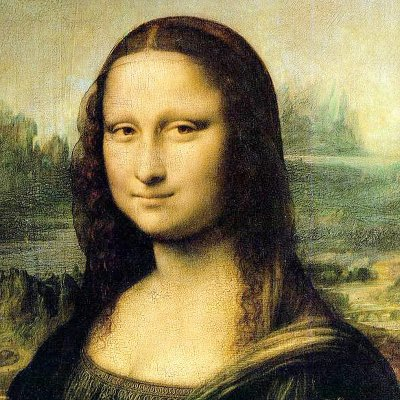
\includegraphics[width=6cm,height=6cm]{mona.jpg}  
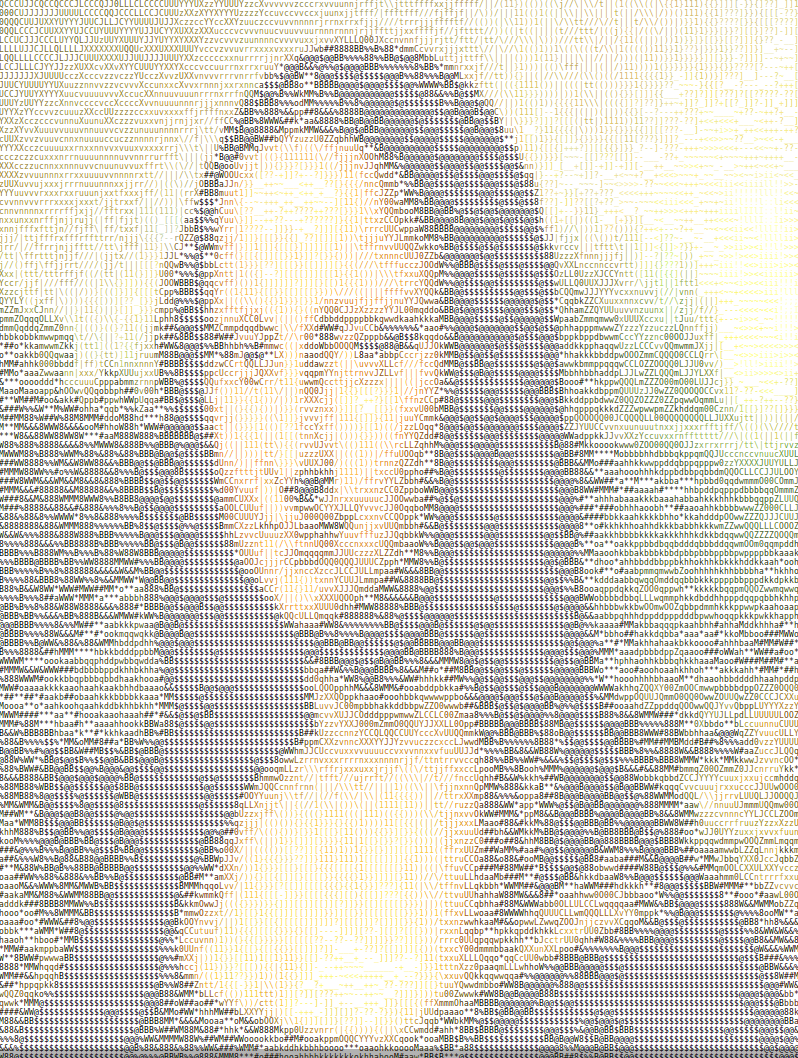
\includegraphics[width=6cm,height=6cm]{monaoutputed.png}
\\ %\caption{Transformation en caractère ASCII avec couleurs.}
\textsc{Figure 2} - Transformation en caractère ASCII avec couleurs
\end{center}

De la même manière pour transformer une image d'Homer Simpson en trames en niveaux de gris il suffit d'exécuter la commande suivante :\verb# ./ascii_art -color 3 /chemin/vers/homer.png#. \\\\
\begin{center}
\centering

\includegraphics[width=7cm,height=8cm]{homer.jpg}
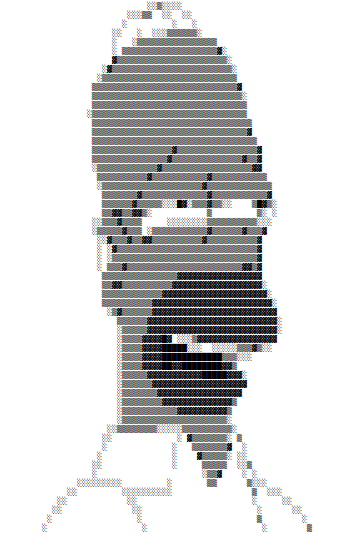
\includegraphics[width=7cm,height=8cm]{homeroutputed.png}
\\ \textsc{Figure 3 -}Transformation en niveaux de gris avec trames.
\end{center}
\section{Idées d'amélioration}
La première idée d'amélioration consiste à pousser encore plus loin la retourche de l'image en entrée en incluant un script auxiliaire ou en faisant appel à une commande de traitement d'images plus poussée que convert. Une autre idée consiste à trier toute la table des caractères ASCII et laisser à l'utiliser le choix de ceux qu'il veut utiliser. 
\newline

Actuellement, la table de caractères utilisée pour représenter les différents niveaux de gris est triée par densité; on pourrait effectuer ce tri de façon automatisé en générant les images correspondant aux caractères en noir et blanc, et en calculant la proportion de pixels noirs. Ceci nous donnerait la densité du caractère en question et permettrait un nouveau tri de la table. 
\end{document}
